%!TEX TS-program = ../make.zsh

\subsection{Technical Issues and Optimizations}
\label{sec:technical_issues_and_optimizations}

Running a simulation with millions of photons propagating and scattering, has to meet certain performance requirements that make sure that the simulations of interest can be run in a reasonable time on current hardware. On the other hand, current graphics processing units (GPUs) afford the opportunity to utilize parallelization capabilities. Both impose technical challenges.
To deal with the necessary complexity and, in particular, to make sure that a complex algorithm does what it is supposed to do, unit tests and cross checks are used as will be described in the next section \ref{sec:unit_tests_and_cross_checks}.
This section focuses on dealing with computational limits, introducing the techniques of GPU parallelization, cluster parallelization, thinning, and performance optimizations.


\paragraph{Simulation-Step Parallelization}
Each simulation step consists of only a few operations: Scattering the photon, checking for absorption, checking for collision with a detector module, and propagating the photon to the next scattering position (see \ref{sec:standard_photon_propagation_algorithm}). This small set of operations can be parallelized, performing the same calculations and operations simultaneously for several thousands of simulation steps, each with different values such as coordinates and directions, on graphics processing units, which are designed for exactly this kind of work. Figure \ref{fig:Id3ioyie} illustrates this parallelization of simulation steps.

\begin{figure}[htbp]
  %\image{dima-parallel-photons-Id3ioyie}
  \hspace{1.5cm}
  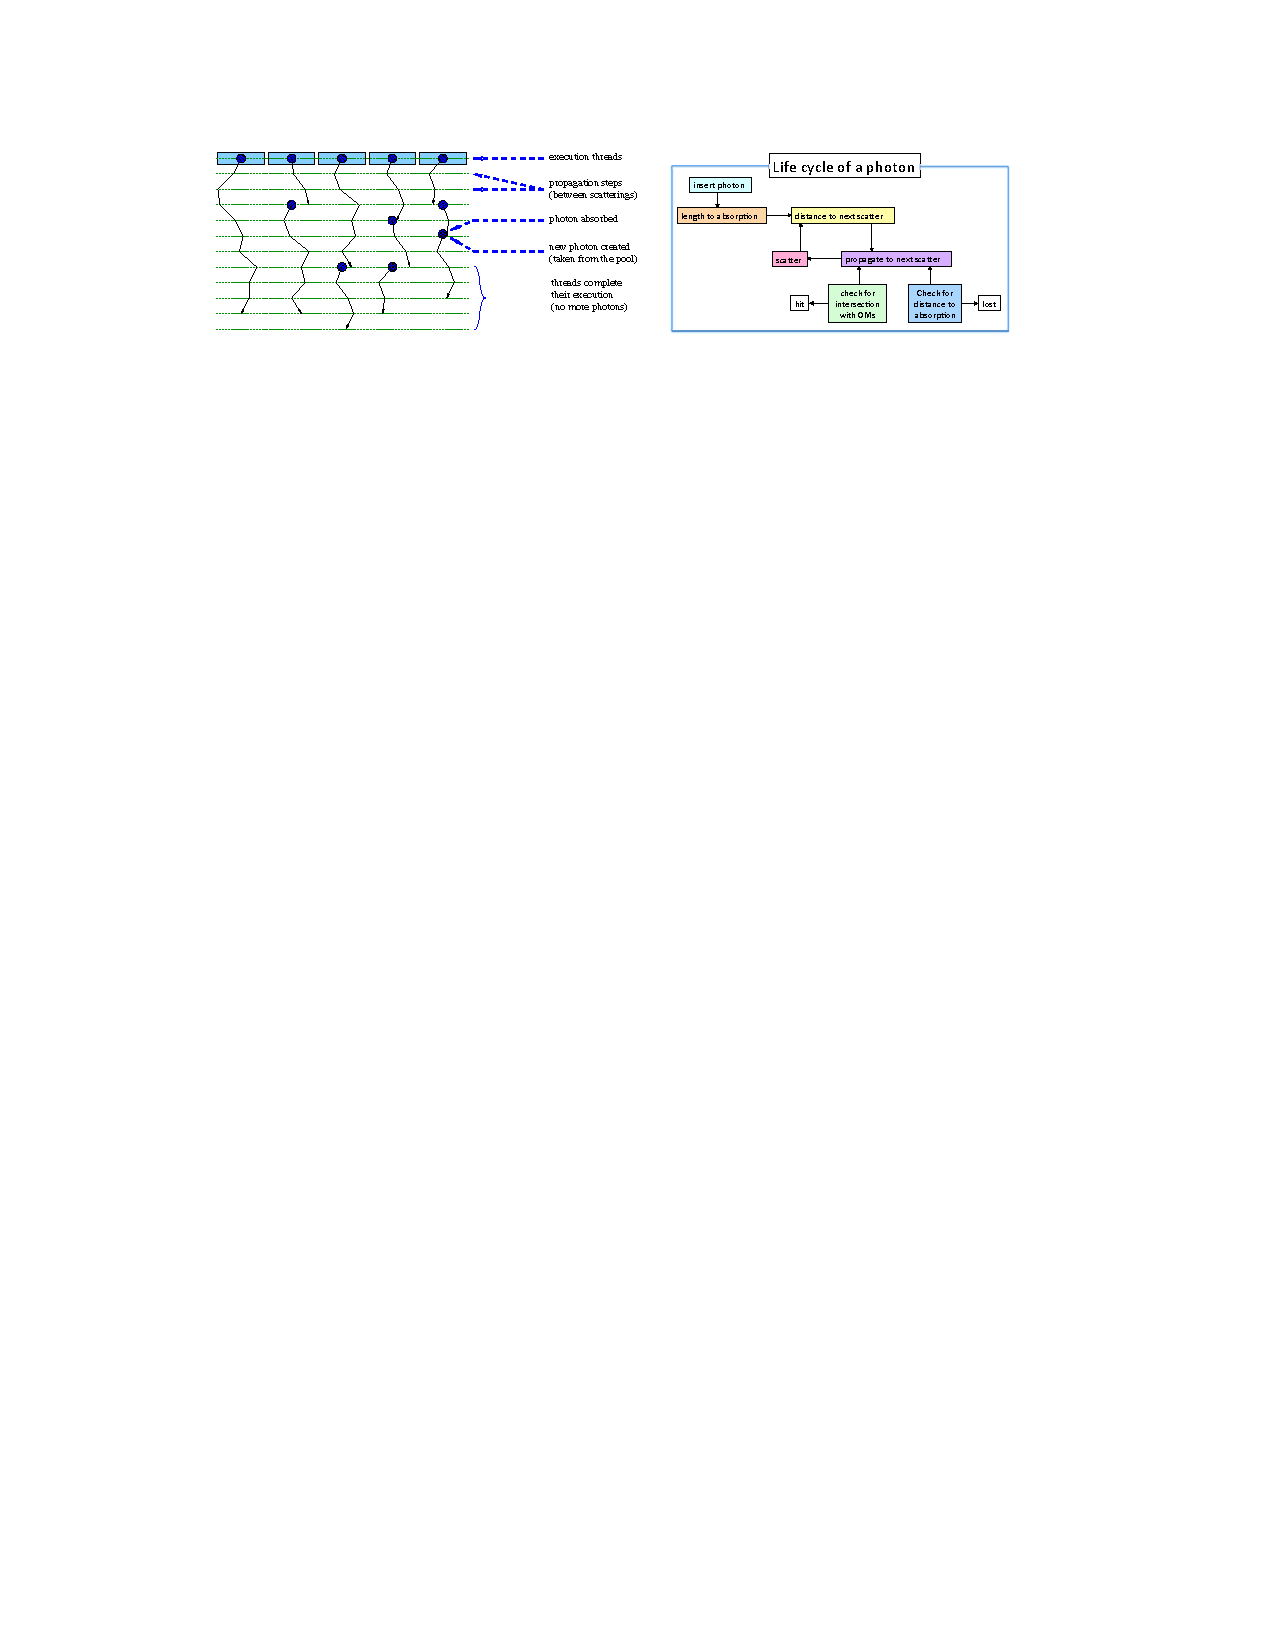
\includegraphics[width=0.7\textwidth, trim={7.7cm 0 0 0}, clip]{img/dima-parallel-photons-Id3ioyie}
  \newline\hspace*{1.5cm}
  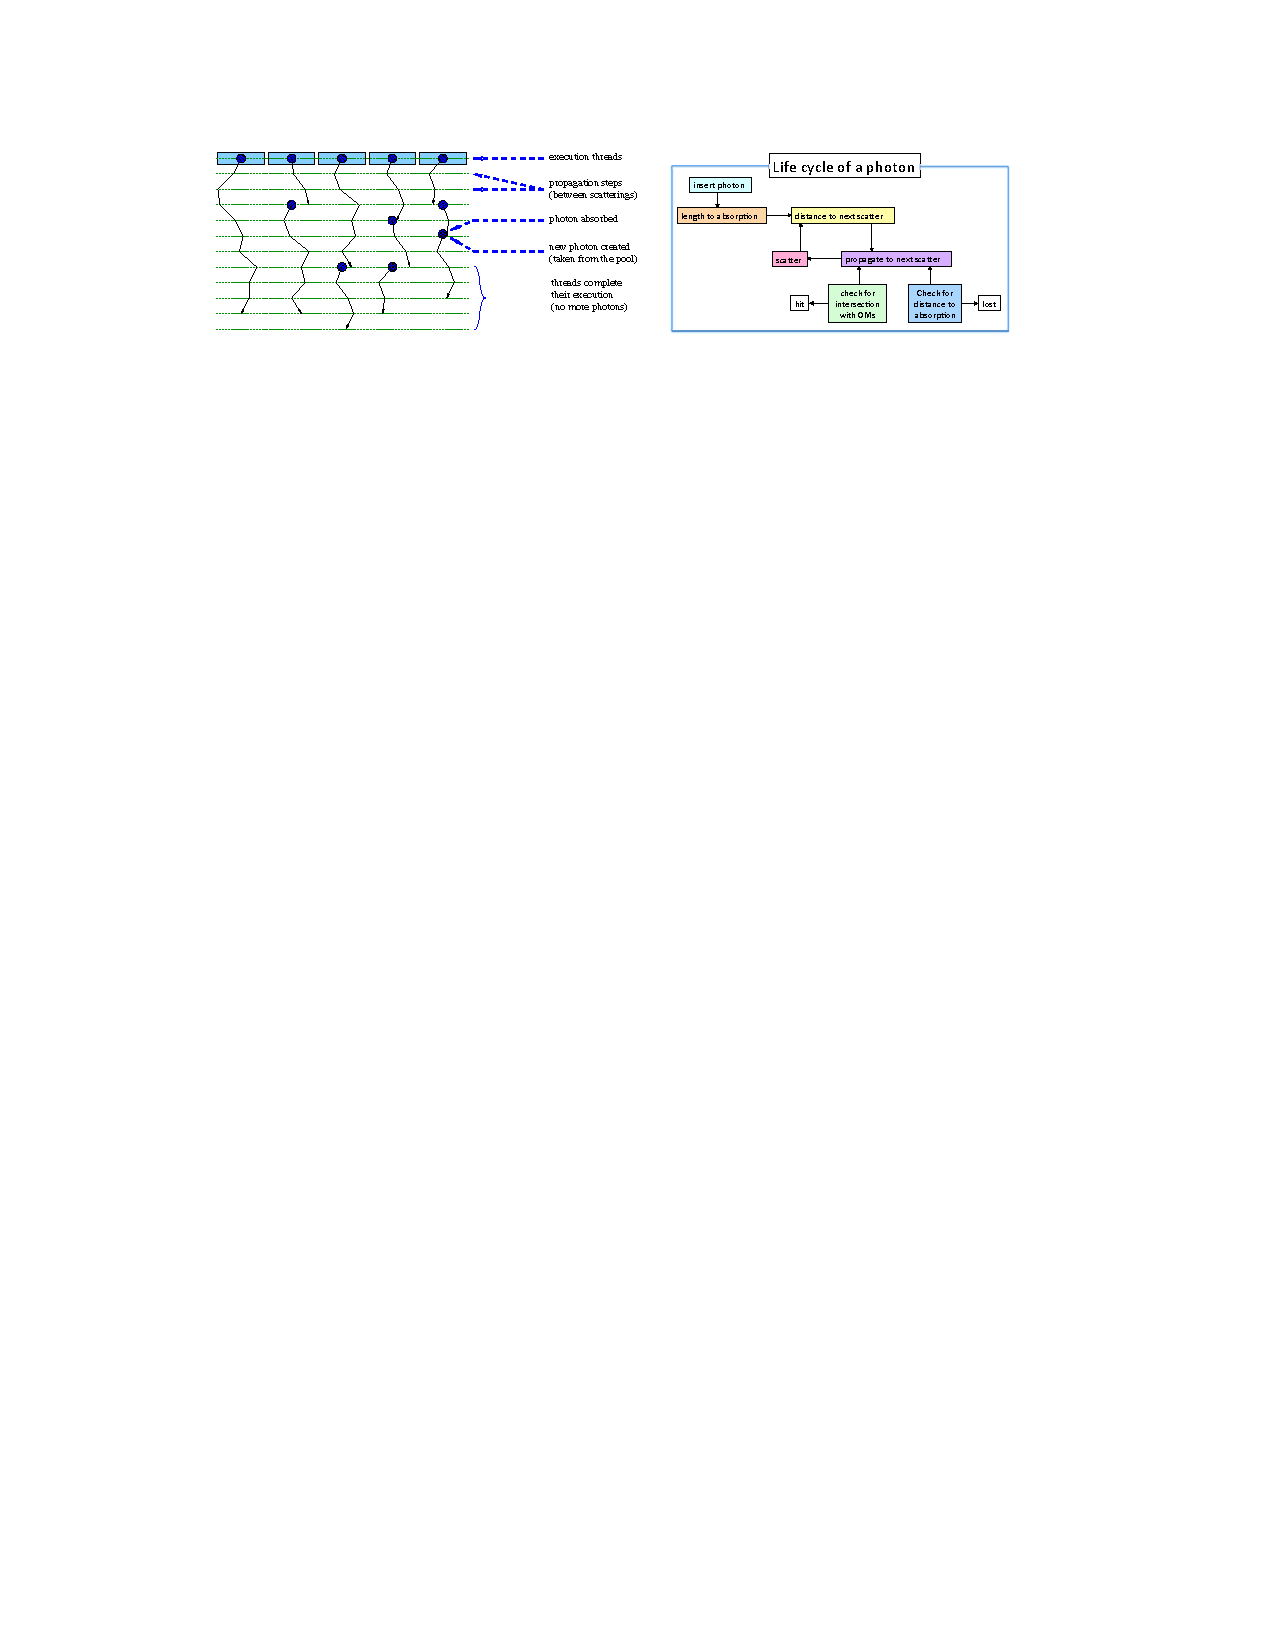
\includegraphics[width=0.9\textwidth, trim={0 0 6.2cm 0}, clip]{img/dima-parallel-photons-Id3ioyie}
  \caption{Parallelization of simulation steps: Tracking of photons entails the computationally identical steps: Propagation to the next scatter, calculation of the new direction after scatter, and evaluation of intersection points of the photon track segment with the detector array. These same steps are computed simultaneously for thousands of photons. (Image and caption taken from \cite{ppcpaper}, figure 1.)}
  \label{fig:Id3ioyie}
\end{figure}

This parallelization leads to a performance improvement by factors of 150 and more when running the propagation simulation on a single GPU compared to running the same simulation on a single CPU core \cite{ppcpaper}.
Standard \clsim as well as the hole-ice extended \clsim can be run on CPUs, GPUs, or both using \noun{OpenCL} as abstraction layer.
In practice, simulating 1000 photons for visualization purposes and recording their paths, which requires a lot of memory, works best on a CPU. Simulating millions of photons, but only recording their final position, where the photon is absorbed within the ice or has it an optical module, works best on GPUs.


\paragraph{Cluster Parallelization}
\label{sec:cluster_parallelization}
A different technique, which adds another layer of parallelization on top of the simulation-step parallelization, is to run the same simulation on a cluster of machines, each equipped with one ore several GPUs. Each machine runs the same simulation, but with different parameters, such as different radii and scattering lengths of the hole-ice cylinders.
This study uses this technique for parameter scans (sections \ref{sec:parameter_scan} and \ref{sec:flasher}) where the same simulation is performed for different parameter sets in order to find a specific parameter set which best fits some kind of external requirement.


\paragraph{Issues Concerning Graphics Processing Units}
Running and developing a simulation software for graphics processing units poses challenges specific to this architecture. A list of technical issues to watch out for in follow-up studies is provided in appendix \ref{sec:gpu_technical_issues}.


\paragraph{Parallel-Programming Optimizations}
% https://github.com/fiedl/hole-ice-study/issues/76
Applying parallel-programming optimization techniques listed in section \ref{sec:parallel_computing} may help to improve the performance of the algorithm that runs on the graphics processing units.

When optimizing code, \noun{Ahmdal's Law} gives the theoretical limit on how much a process can be sped up by optimizing one of its components. \cite{raytracingtips}

$$ s_\text{total} = \frac{1}{(1 - p) + \sfrac{p}{s_\text{comp}}}, \ \ \ s = \frac{t_\text{before}}{t_\text{after}}, \ \ \
\lim_{s_\text{comp}\rightarrow\infty} s_\text{total} = \frac{1}{1-p} $$

Here, $s_\text{total}$ is the resulting speedup of the whole process, which is defined as the fraction of the time the process takes before the optimization and the time the same process takes after the optimization has been applied. $p$ is the portion of execution time that the component requires before optimizing. $s_\text{comp}$ is the speedup the the component that is optimized achieved by the optimization.
Even in the limit that the component that is optimized takes zero time after applying the optimization, $s_\text{comp}\rightarrow\infty$, the speedup of the whole process is limited.
Also, \authorname{House} and \authorname{Wyman} \cite{raytracingtips} recommend to first write working code, and then optimize in a second step.

One important key concept to efficient parallel programming is to avoid executional threads being idle, waiting for other threads to finish before resuming.
One application of this concept in the hole-ice algorithm is to \textbf{filter hole-ice cylinders by range} in a \textbf{separate loop}.
The algorithm needs to check in each simulation step, which hole-ice cylinders are in range of the photon and therefore should be considered when calculating the propagation through the hole ice. Without this optimization, the cylinders are processed one by one in each simulation step. While, in each iteration of the cylinder loop, all photons in range of one specific cylinder are propagated through that cylinder, all other photons not in range of the cylinder, wait idly and thereby waste computation time. This is illustrated in figure \ref{fig:ceiV8Yai} (a).

Even though the optimization adds time for the additional loop where the indices of the cylinders in range are saved into a local array, the main loop where the propagation through each cylinder is handled is much faster now, because it does not need to iterate over all cylinders in the detector but only over the cylinders in range of the photon and improves parallelization as illustrated in figure \ref{fig:ceiV8Yai} (b).

\docpar{The implementation of this optimization is documented in \issue{30}.}

\begin{figure}[htbp]
  \subcaptionbox{Checking if a cylinder is in range in the same loop as propagating through that cylinder. The cylinders are processed successively. Lots of photons are idle.}{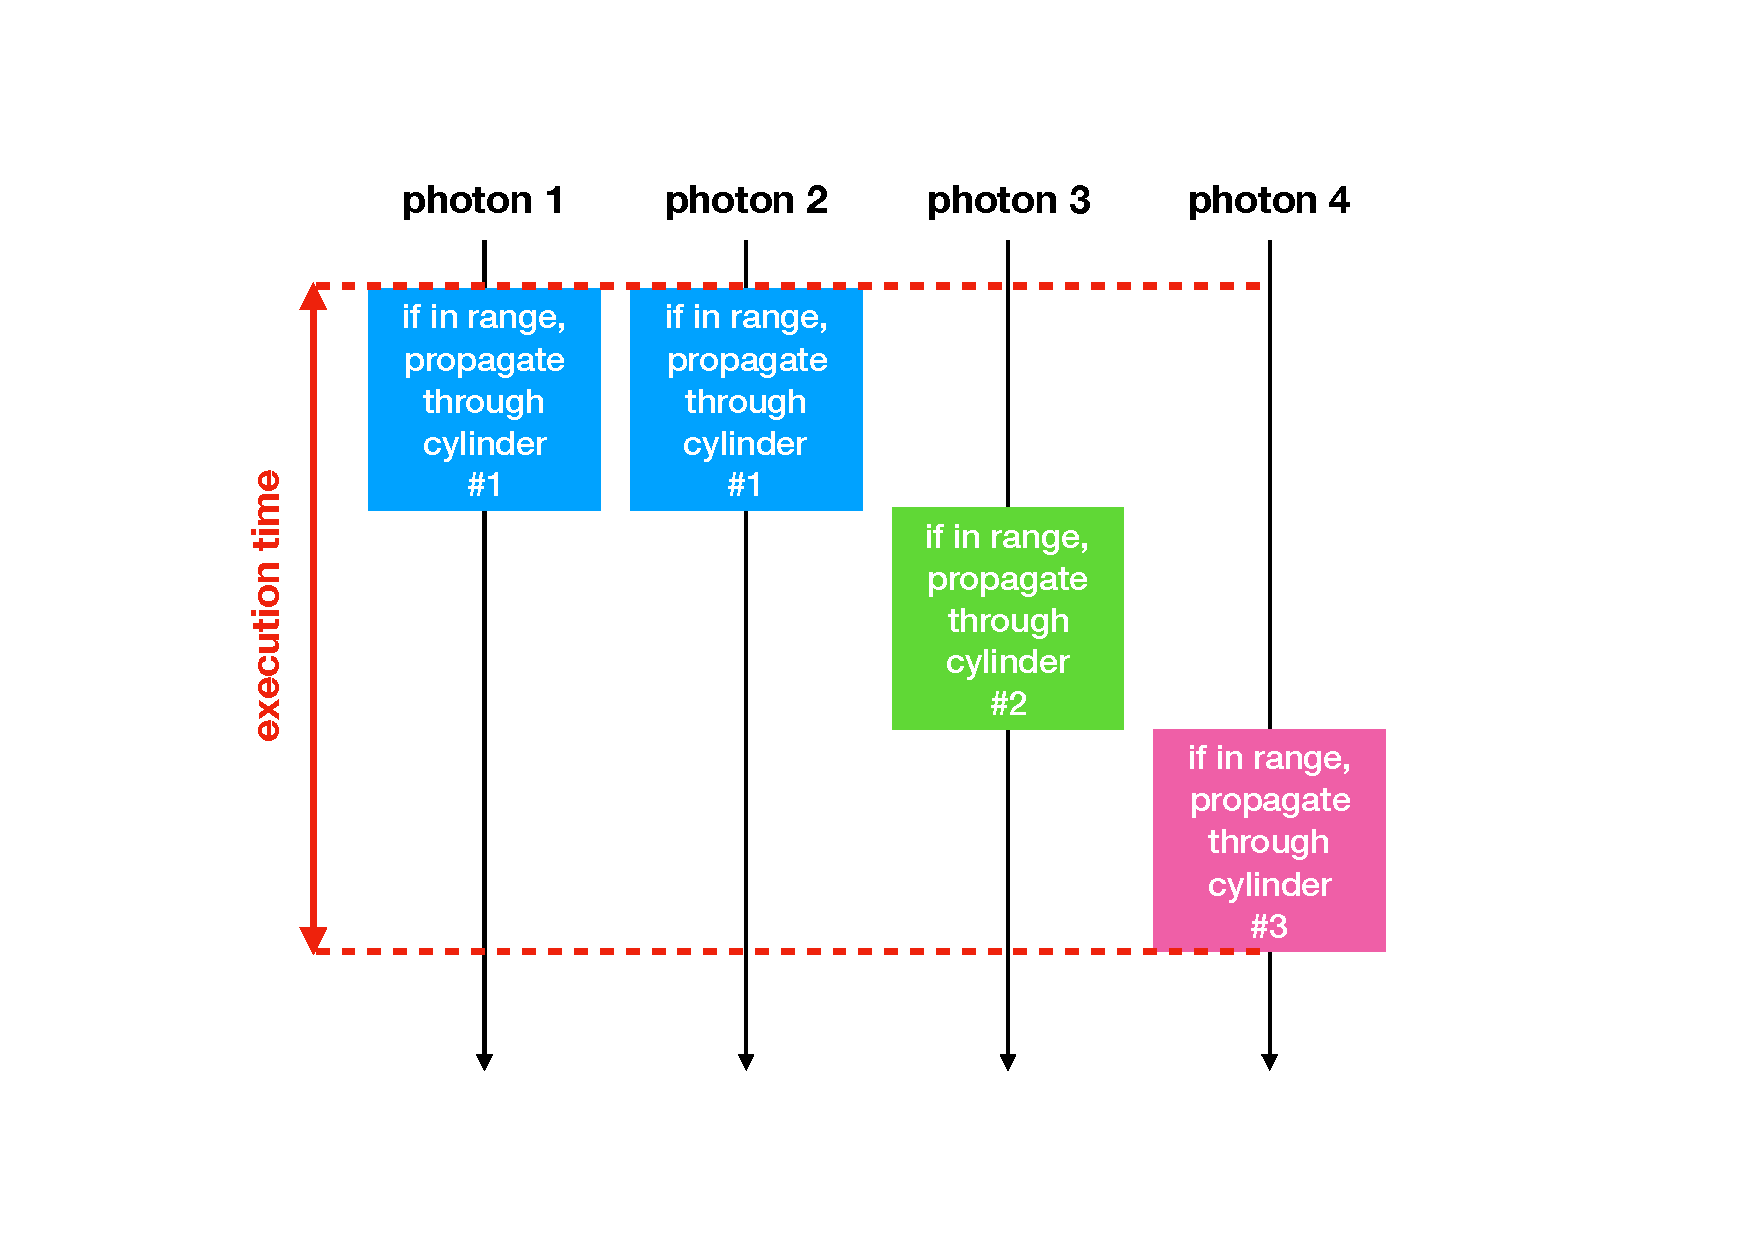
\includegraphics[width=0.48\textwidth, clip, trim = {4cm 2cm 6cm 2cm}]{img/cylinder-sort-ceiV8Yai}}\hfill
  \subcaptionbox{Checking if a cylinder is in range in a separate loop. The main loop where the photons are propagated through the cylinders does not loop over all cylinders but only over cylinders marked as in range for each photon respectively. }{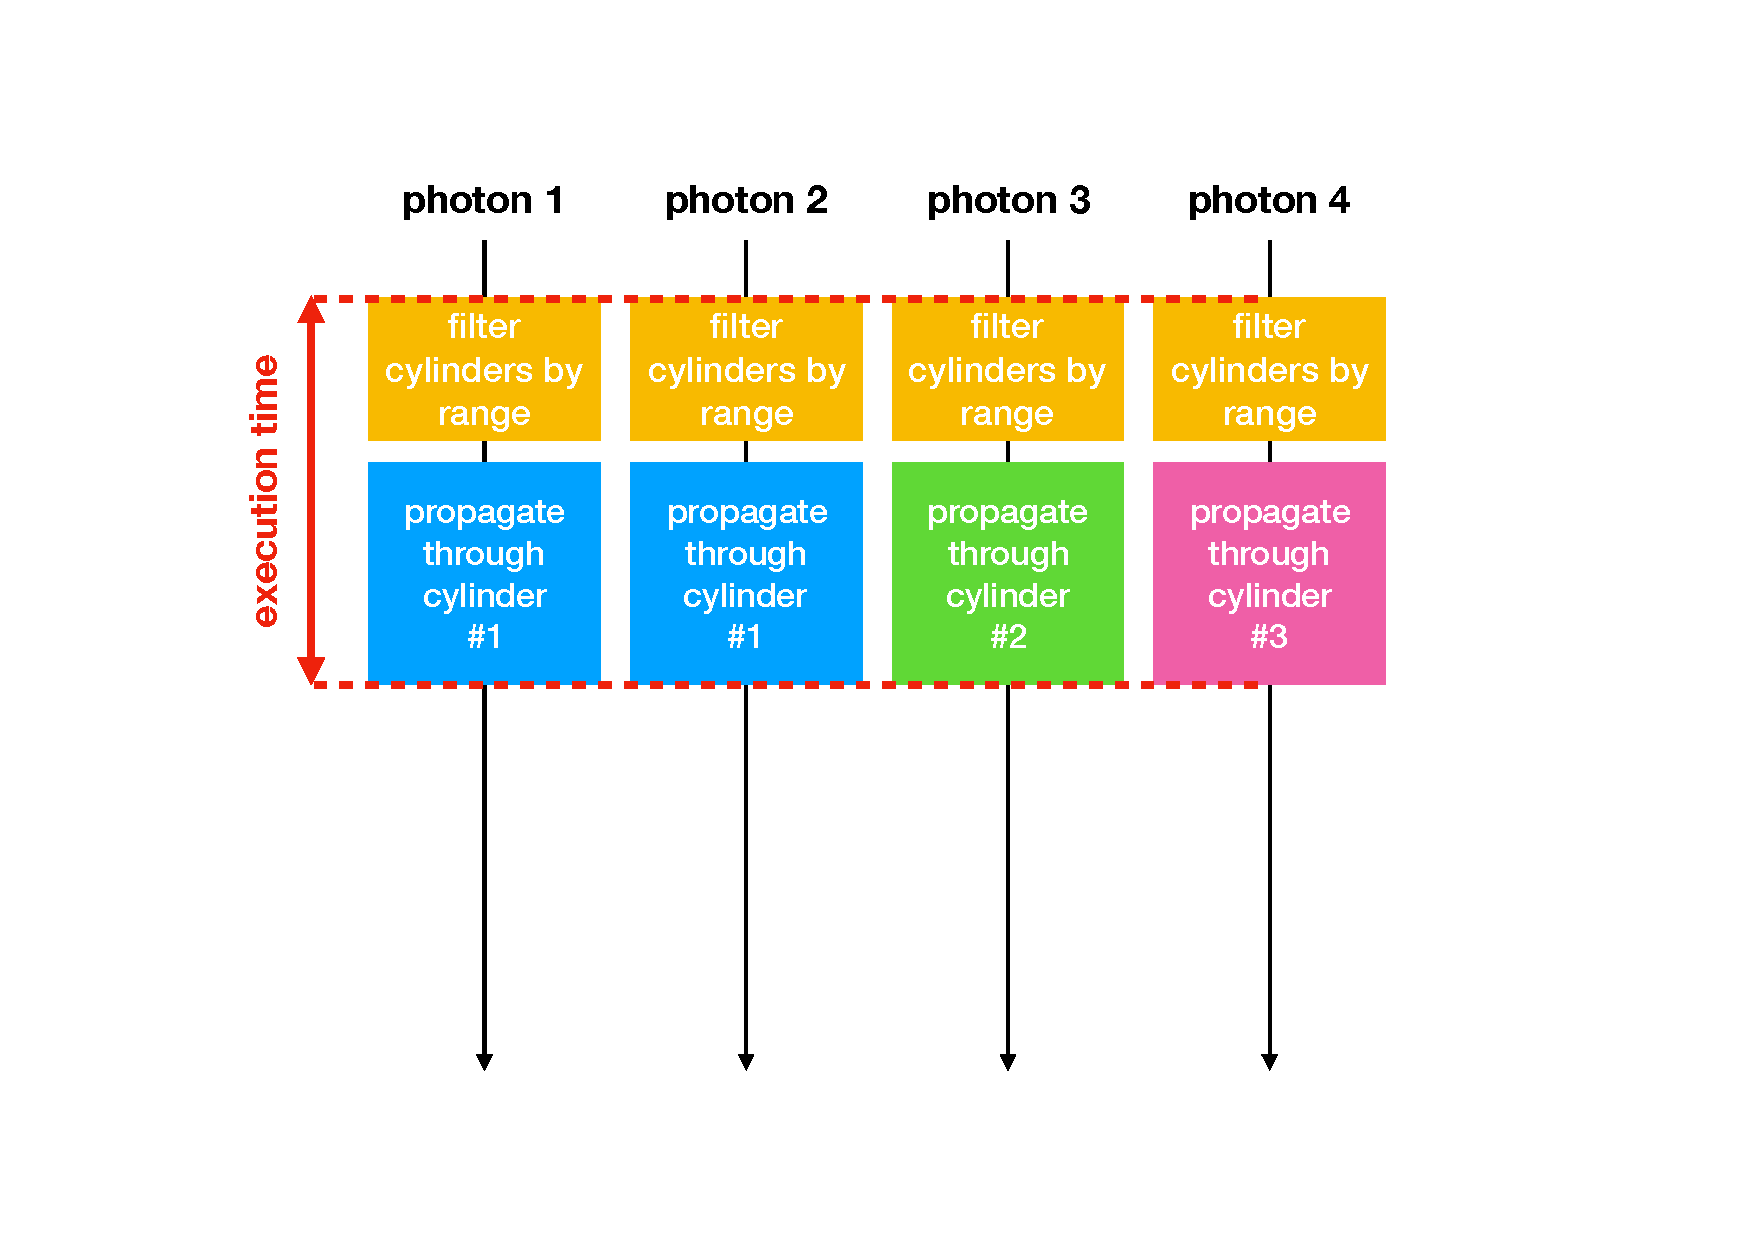
\includegraphics[width=0.48\textwidth, clip, trim = {4cm 2cm 6cm 2cm}]{img/cylinder-sort-compact-ceiV8Yai}}
  \caption{Processing the propagation of photons through hole-ice cylinders in parallel. While filtering cylinders by range separately adds additional executional time, it improves parallelization and thereby saves execution time overall.}
  \label{fig:ceiV8Yai}
\end{figure}


Another optimization used in the hole-ice algorithm is to \textbf{order mathematical cases by their frequency of application}. In a case-by-case analysis, each executional thread skips the additional case checks when its case is determined. If the checks for common cases are handled first, there is a good chance that all of the parallel threads fall into common cases such that the checks for the rare cases can be skipped for the whole thread block.
This technique is used in the implementation of the geometric cases for both the hole-ice-correction algorithm (\ref{sec:algorithm_a}) and the new media-propagation algorithm (\ref{sec:algorithm_b}).


\paragraph{GPU-Specific Optimizations}
In addition to the general principles of parallel programming (section \ref{sec:parallel_computing}), \authorname{House} and \authorname{Wyman} \cite{raytracingtips} list practical tips for optimizing GPU-ray-tracing code.
Most notably, passing data structures by reference rather than by value proved to have significant performance impact because \textbf{allocating memory on a GPU is expensive}. This also includes simple structures like arrays of numbers, and even re-using the same array for several calculations rather than re-defining it. This technique has caused a performance improvement on GPUs by a factor of six in this study.

\docpar{This optimization of re-using arrays is documented in \issue{70}.}

\textbf{Optimizing mathematical operations} on paper is an important technique as each calculation operation that can be cut down on in a procedure that saves time when executing the procedure many times. In addition to simplifying equations mathematically, avoiding numerically expensive operations such as square roots improves performance.

GPUs support 4-dimensional vectors as native data types as well as native vector operations such as the dot product. Expressing equations in terms of vectors rather than simplifying equations on the coordinate level, resulted in improved performance and numerical accuracy.

\docpar{This optimization of using vector types rather than scalar types is documented in \issue{28}.}


\paragraph{Performance Profiling}
\authorname{Owens} recommends profiling tools like \noun{gprof}, \noun{VTune}, or \noun{VerySleepy} \cite{cudacourse}. But also basic techniques like printing time differences between executional blocks can help to isolate performance problems. Figure \ref{fig:profiling-paz4Eig6} shows the execution time profile of the simulation step of the new medium-propagation algorithm.

Note that printing a profiling result may be more expensive as the computation that is to be profiled itself. In this study, printing the time difference of the beginning and the end of a simulation step takes five times as long as the simulation step itself.

\docpar{Profiling the simulation step is documented in \issue{69}.}

\begin{figure}[htbp]
  \image{profiling-paz4Eig6}
  \caption{Performance profile of the average simulation step in arbitrary units (GPU clock cycles). Each row of the chart represents a different algorithm. In the first row, which shows an early stage of the new medium-propagation algorithm, the initial memory allocation within each simulation step takes a lot of time, especially when comparing to standard \clsim (row 3). The second row shows the profile of the new medium-propagation algorithm after a memory issue has been fixed. Notable operations in each simulation step are the initial memory allocation for local variables, adding ice layers, adding hole-ice cylinders, sorting medium boundaries by distance to the photon and looping over the media to convert the interaction budget into geometrical distances.}
  \label{fig:profiling-paz4Eig6}
\end{figure}


\paragraph{Performance Optimizations for Production Use}
After implementing and debugging a new algorithm, a lot of debug outputs and other development tools are no longer required when running simulations. For those production simulations, the debug features can be turned off by \textbf{compiling the \icecube simulation framework for production} use rather than for debugging. Thereby, simulations run significantly faster as debug outputs often cost more time than the actual simulation itself.

\docpar{How to switch between a debug build and a production build is documented in \issue{73}.}

Also, activating \textbf{kernel caching} on the production machines may improve simulation performance. However, this should only be used when always using the same propagation kernel, and should be avoided when switching between kernel versions or turning kernel features on and off, because the kernel cache will not be reliably reset automatically when changing kernels.

\docpar{How to enable or disable kernel caching is documented in \issue{15}.}

\label{sec:thinning}
Another way to save computational time when performing simulations, especially large cluster scans, is to scale down the number of photons using a \textbf{thinning factor}. A representative fraction of the photons is propagated in the simulation, and then the simulation results, for example the numbers of hits in each detector module, are scaled up accordingly.

\docpar{This thinning technique is used in the flasher parameter scan documented in \issue{59}.}
